\documentclass[manuscript]{aastex}

\usepackage{float}
\bibliographystyle{apj}

\begin{document}

\title{Positional Abudance Trends in Red Clump Star in the Milky Way}
\author{Natalie Price-Jones}

\section{Background}
\label{sec:back}
The question of galaxy formation is a relatively open one. Although simulations have succeeded in tracing the broad strokes of formation history, there are subtle connections between elements in a galaxy whose evolution is not yet well understood. Observational evidence implies empirical relations between properties of different bulk components of galaxies, like bulge and disk velocity dispersion, as well as correlations between large and small scales, such as the $M_{\rm BH}-\sigma$ relation. Some of these observations also serve as indirect evidence for dark matter, but the detailed influence of this elusive substance on a galaxy's dynamical history is not known. Understanding a galaxy's formation history offers an opportunity to investigate the source of these relations and may allow for predictions about how galaxies will continue to evolve and interact.

In distant galaxies, we may study a galaxy's bulk properties, but our position in the Milky Way offers us the opportunity to examine individual stars of our own galaxy in detail. These individual elements at small scales are influenced by bulk properties, the dynamical evolution of the galaxy. By searching for correlations in properties including effective temperature, gravitational acceleration and elemental abundances we can learn about where and how populations of stars form and what happens to them over their lifetimes. 

Finding this information relies on stellar surveys that extend far beyond the solar neighbourhood. Large-volume spectroscopic survey data from the APO Galactic Evolution Experiment (APOGEE), the Large Sky Area Multi-Object Fibre Spectroscopic Telescope (LAMOST) and upcoming data from the Gaia mission will offer rich and detailed information about hundreds of thousands of stars. Even with data reduction pipelines in place, interpreting that data to find meaningful results will be challenging. However, these results might offer constraints on theories of the Milky Way's formation and evolution, which in turn hints at similar processes at work in other galaxies.  


\section{Research Plan}
\label{sec:rp}

In the broadest sense, this project will attempt to address some of the questions raised in \S\ref{sec:back} about galaxy formation through analysis of Milky Way stars. Previous work \citep{bovy2015} has found that comparing alpha-element abundance [$\alpha$/Fe] to metallicity [Fe/H] reveals two distinct populations: a main trendline, with another population that has an enhancement above this line in $\alpha$ elements (O, Mg, Si, S, Ca, Ti): see Figure \ref{fig:abun}. We will investigate individual $\alpha$ elements, as well as the other 8 elemental abudances, for similar correlations, and trace where these stars are located within the galaxy (radially and vertically). Stars falling into the same small bins in all elemental abundances we call mono abundance populations (MAPS). Classifying such populations may make it possible to trace migratory motion of stars over the course of their lifetimes, knowing that stars with similar elemental abudances likely had similar formation environments.

\begin{figure}%[H]
\centering
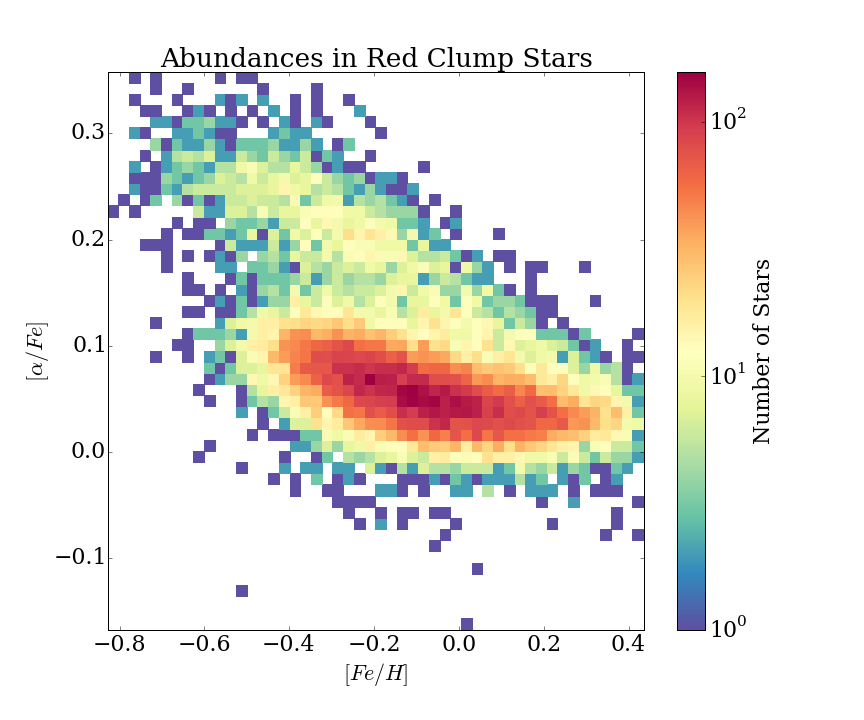
\includegraphics[width = 0.8\linewidth]{alpha_vs_fe.png}
\caption{$\alpha$-enhancement vs iron abundance for 19936 red clump stars from APOGEE Data Release 12.}
\label{fig:abun}
\end{figure}

\subsection{Data Set}
\label{sec:data}
This work will focus analysing the spectra of a sample of red clump stars from APOGEE's Data Release 12. These stars are selected according to cuts in gravity, effective temperature, and metallicity, and leave us with a sample of 19936 stars. These stars trace, to some extent, the stellar population of the Milky Way through the volume of the APOGEE survey. A star's time in the red clump is short compared to its lifetime, so the sample is biased towards locating younger stars. Data on these stars comes in the form of infrared (H-band) spectra covering a wavelength range from 1.514 $\mu$m to 1.696 $\mu$m (with some small nm gaps between detectors). APOGEE's DR12 pipeline provides data on abundances of 15 elements (C, N, O, Na, Mg, Al, Si, S, K, Ca, Ti, V, Mn, Fe, Ni) as well as effective temperature ($T_{\rm eff}$), surface gravity ($\log(g)$) and alpha-element enhancements ([$\alpha$/Fe]).

\subsection{Methods}
\label{sec:methods}

In order to have confidence in our elemental abudances, we must remove other effects from the stellar spectra. We will start by fitting each pixel with a polynomial in stellar parameters $T_{\rm eff}$, $\log(g)$ and $[Fe/H]$, and calculate the residuals of this fit in pixels corresponding to absorption features corresponding to particular elements. A sample of stars from globular clusters observed by APOGEE and analyzed by \citet{meszaros2015} will undergo the same fitting to make an estimation of the intrinsic scatter in this residual measurement. Stars from the same cluster are expected to have low variation in abudances, having all formed in the same environment, and so provide a good comparison baseline. This fitting method is straightforward, but a more sophisticated method of modelling stellar parameters may later be used \citep{ness2015}.

\bibliography{cite}

\end{document}